\documentclass[tikz,border=1pt]{standalone}

\usepackage{amsmath}
\usepackage{xcolor}
\usepackage{tikz}
\usepackage{helvet}
\renewcommand{\familydefault}{\sfdefault}  % Set sans-serif as default

\usetikzlibrary{arrows.meta}
\usetikzlibrary{calc, fit, matrix, positioning}

\tikzstyle{circ}=[circle, draw, minimum size=1.2cm]
\tikzstyle{square}=[rectangle, draw, minimum size=1.2cm]

\begin{document}

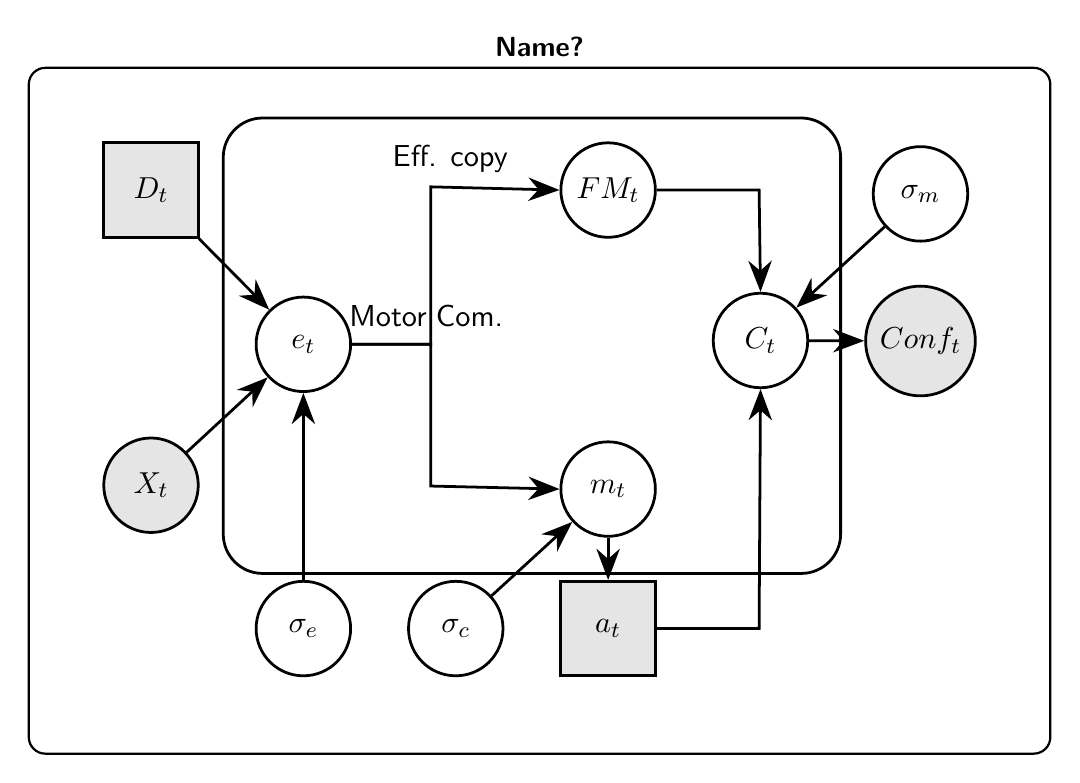
\begin{tikzpicture}

\tikzset{>={Stealth[scale=1.5]}}
\tikzset{every node/.style={font=\sffamily\fontsize{11pt}{12pt}\selectfont}}
\tikzset{every path/.style={line width=1pt}}

% Main matrix
\matrix (m0) [
    ampersand replacement=\&,
    matrix of math nodes,
    nodes in empty cells,
    column sep=.7cm,
    row sep=0.5cm,
]
{
    |[square, draw, fill=gray!20]| D_t \& 
    |[minimum size=1.2cm, inner sep=0pt, draw=none]| \&
    |[minimum size=1.2cm, inner sep=0pt, draw=none]| \&
    |[circ, draw]| FM_t \&
    |[minimum size=1.2cm, inner sep=0pt, draw=none]| \&
    |[circ, draw]| \sigma_m \\
    |[minimum size=1.2cm, inner sep=0pt, draw=none]| \&
    |[circ, draw]| e_t \&
    |[minimum size=1.2cm, inner sep=0pt, draw=none]| \&
    |[minimum size=1.2cm, inner sep=0pt, draw=none]| \&
    |[circ, draw]| C_t \&
    |[circ, draw, fill=gray!20]| Conf_t \\
    |[circ, draw, fill=gray!20]| X_t \&
    |[minimum size=1.2cm, inner sep=0pt, draw=none]| \&
    |[minimum size=1.2cm, inner sep=0pt, draw=none]| \&
    |[circ, draw]| m_t \&
    |[minimum size=1.2cm, inner sep=0pt, draw=none]| \&
    |[minimum size=1.2cm, inner sep=0pt, draw=none]| \\
    |[minimum size=1.2cm, inner sep=0pt, draw=none]| \&
    |[circ, draw]| \sigma_e \&
    |[circ, draw]| \sigma_c \&
    |[square, draw, fill=gray!20]| a_t \& 
    |[minimum size=1.2cm, inner sep=0pt, draw=none]|  \\
};

% Arrows for motor system and efference copy
\draw[->] (m0-1-1) -- (m0-2-2); % D_t -> e_t
\draw[->] (m0-3-1) -- (m0-2-2); % X_t -> e_t
\draw[->] (m0-4-2) -- (m0-2-2); % sigma_e -> e_t
\draw[->] (m0-3-4) -- (m0-4-4); % m_t -> a_t
\draw[->] (m0-4-3) -- (m0-3-4); % sigma_c -> m_t
\draw[->] (m0-2-5) -- (m0-2-6); % C_t -> Conf_t
\draw[->] (m0-1-6) -- (m0-2-5); % sigma_m -> Conf_t
\draw[->]  (m0-1-4.east) -- ++(--1.3cm,0) -- ++(0,0cm) -- (m0-2-5.north); % FM_t -> FM_t
\draw[->]  (m0-4-4.east) -- ++(--1.3cm,0) -- ++(0,0cm) -- (m0-2-5.south); % m_t -> FM_t
\draw[->]  (m0-2-2.east) -- ++(--1cm,0) -- ++(0,2cm) -- (m0-1-4.west); % e_t -> FM_t
\draw[->]   (m0-2-2.east) -- ++(--1cm,0) -- ++(0,-1.8cm) -- (m0-3-4.west); % e_t -> m_t

% Trial plate
\pgfsetcornersarced{\pgfpoint{5mm}{5mm}}
\node[draw=black, fit=(m0-1-2) (m0-3-5), inner sep=4mm] {};

\node[rotate=0, anchor=west] at (-2,3.2) {Eff. copy};
\node[rotate=0, anchor=west] at (-2.55,1.2) {Motor};
\node[rotate=0, anchor=west] at (-1.45,1.2) {Com.};


\node[
  draw,
  thick,
  rounded corners=6pt,
  fit=(m0),
  inner sep=8mm,
  label={[font=\bfseries]above: Name?},
  name=wholemodel
] {};

\end{tikzpicture}
\end{document}